\documentclass{ctuthesis}
\ctusetup{
    xdoctype = B,
    xfaculty = F3,
    mainlanguage = english,
    titlelanguage = english,
    title-english = {Model of CAN FD Communication Controller for QEMU Emulator},
    title-czech = {Model kontroléru CAN FD v emulátoru QEMU},
	doctype-english = {Bachelor Thesis},
    department-english = {Department of Control Engineering},
    author = {Jan Charvát},
	keywords-czech = {sběrnice CAN, CAN FD, QEMU, Linux, CTU CAN FD, SocketCAN, SJA1000},
	keywords-english = {CAN bus, CAN FD, QEMU, Linux, CTU CAN FD, SocketCAN, SJA1000},
    supervisor = {Ing. Pavel Píša, Ph.D.},
    supervisor-address = {Praha 2\\ Karlovo náměstí 13\\ E-7a},
    day = 21,
    month = 5,
    year = 2020,
    specification-file = {Zadani_Charvat_OI_BP_angl.pdf},
    front-specification = true,
}
\ctuprocess
\usepackage{tabularx, array, booktabs}
\begin{declaration}
I declare that this thesis has been
 composed solely by myself and that it
 has not been submitted, in whole or in
 part, in any previous application for a
 degree. Except where states otherwise
 by reference or acknowledgment, the
 work presented is entirely my own. \\
\\
\\
In Prague,~\ctufield{day}.~\ctufield{month}.~\ctufield{year} \qquad .......................
\end{declaration}
\begin{thanks}
I would like to thank Ing. Pavel Píša Ph.D for tutoring and time investments towards my Thesis.
\end{thanks}
\begin{abstract-english}
 This thesis begins with a theoretical part, which features an analysis of CAN 2.0 and the differences with the newer standard CAN FD. It continues with QEMU CAN subsystem description. The main goal of the thesis is to contribute to QEMU mainline with an implementation of a CAN FD communication bus and model of a CAN FD capable controller (open-source CTU CAN FD in a particular case) as an extension of an already implemented CAN 2.0 capable chip SJA1000 emulation.
\end{abstract-english}

\begin{abstract-czech}
 Tato práce začíná teoretickou částí, která obsahuje analýzu standardu CAN 2.0 a jeho rozdíly s nejnovějším standardem CAN FD. Teoretická část pokračuje s popisem CAN subsystémů v QEMU. Hlavní cíl práce je přispět do vývoje QEMU implementací CAN FD komunikační sběrnice a emulace čipu uzpůsobeného pro CAN FD jako rozšíření již implementovaného CAN 2.0 čipu SJA1000.
\end{abstract-czech}

\begin{document}

\maketitle
\chapter*{Nomenclature}

\noindent
\begin{tabularx}{\linewidth}
  { l >{\raggedright\arraybackslash}X }
\bfseries Acronym  & \bfseries Meaning \\\Midrule
CTU & Czech Technical University \\
FEE & Faculty of Electrical Engineering \\
CAN & Controller Area Network \\
ID & Identifier \\
FD & Flexible Data Rate \\
ECU & Electronic Control Unit \\
PCI & Peripheral Component Interconnect \\
CANH & CAN-Height Line \\
CANL & CAN-Low Line \\
SOF & Start of Frame \\
RTR & Remote Request \\
IDE & Identifier Extension \\
DLC & Data Length Code \\
CRC & Cyclic Redundancy Check \\
ACK & Acknowledgement \\
BRS & Bit Rate Speed \\
FDF & Flexible Data Rate Frame \\
ESI & Error Status Indicator \\
Tx buffer & Stores the Data For Transmission \\
Rx buffer & Stores the Received Data \\
TMP buffer & Temporary Buffer \\
FIFO & First In First Out \\
TXCE & "set\_empty" Command \\
TXCR & "set\_ready" Command \\
TXCA & "set\_abort" Command \\
RXFRC & RX Buffer Frame Count \\
RWCNT & Count of Words in CAN Frame Without FRAME\_FORMAT WORD \\
RRB & Release Rx Buffer \\
IRQ & Interrupt Request \\
RAM & Random Access Memory \\
\end{tabularx}

\chapter{Introduction}
 The goal of this bachelor thesis is to implement a CAN FD communication bus and controller emulation for QEMU full system emulator mode. It builds on previous and ongoing CAN bus related projects developed and coordinated by the CTU FEE. The support of the classic SJA1000 CAN 2.0 controller model for QEMU emulator development started by Jin Yang in RTEMS GSoC 2013 slot. This slot, mentored by Pavel Pisa from the CTU, reached the QEMU mainline in 2018. \cite{qemu-mainline} CTU CAN FD controller \cite{ctu-canfd-core} initiated by Ondrej Ille at the CTU FEE is selected as the device model used by a guest system to access the CAN FD bus variant. The Linux kernel driver for this controller is available as the result of Martin Jerabek's thesis. \cite{ctu-canfd} \\
 The CAN controller core emulation needs to be connected to some type of a system bus in order to be visible to the emulated CPU and the guest system. A model of the commercially available Kvaser PCI addon card is used for the SJA1000 emulation. The PCI Express card integration of CTU CAN FD \cite{ctu-project} has been selected as a goal for this thesis. \\
 SocketCan is used to interface a QEMU emulated CAN bus to the CAN bus of the host system when QEMU is run on the Linux system. The QEMU side of the interface has to be extended to support a CAN FD protocol.
The most significant implementation part of this project is to emulate CTU CAN FD IP core register map \cite{progdum} with QEMU, to get the communication through these emulated hardware parts on a real CAN hardware bus, and to see this communication on the other side by monitoring tools. \\
This project is open-source, corresponding to the whole QEMU. \\
My focus on the CAN bus stems from my participation in one external company project, which which delivers utilities for trains where CAN communication is used.

\chapter{CAN}
 Automotive industry often uses CAN.  For instance, almost every car uses a CAN bus. One of the reasons is the need to avoid carrying hundreds of kilograms of wire in the car. CAN enables the connection between several ECUs via one bus \cite{ECUs}, instead of many analog signal lines. Another advantage lies in the fact that all CAN nodes receive each message and decide whether they want to utilize it or not. However, the application spectrum is broad. CAN was standardized by the Bosch company in 1986; hence, industry needs and CAN development have been making a significant progress. This bachelor thesis concentrates on CAN FD, the latest and most significant innovation in CAN technology.

 \section{CAN 2.0}
  ISO 11898-1:2003 describes CAN 2.0. The picture below shows the configuration of the individual bits within the frame. It is apparent that in order to send 8 bits of data, the overhead is quite significant. 
  \begin{figure}[H]
  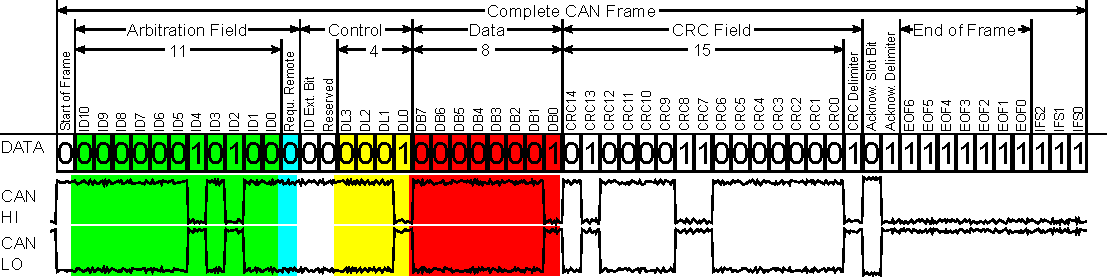
\includegraphics[width=1\textwidth]{CAN-Bus-frame_in_base_format_without_stuffbits}
  \caption{CAN frame detail \cite{can_frame}}
  \end{figure}
  The frame starts with SOF, which is always dominant zero. It serves to notify other CAN nodes at the arbitration’s start of a new frame being sent. Then comes the identifier, CAN 2.0 brings two length variants for ID, CAN 2.0a corresponds to a sample image and has an 11-bit identifier. CAN 2.0b standard extends the identifier to 29-bit. RTR in dominant zero marks the standard frame; in the recessive state, it changes into a Remote frame, which requests data from a CAN node with the corresponding ID assigned to the identifier place. IDE distinguishes between the standard and extended ID format. DLC holds data bytes count that is a number between 0 and 8 bytes per message and the respective data are saved immediately afterwards. CRC serves as a data integrity check. ACK first bit is the space for confirmation that at least one CAN node has accepted the message and the second bit for the information that at least one CAN node has not accepted the message correctly. If the second condition is achieved, the whole frame is resent automatically.
  \subsection{Physical layer}
   CAN physical layer consists of twisted pair cabling CANH and CANL. The logic value is calculated as the result of CANH - CANL and is labelled as Vd \cite{can_Vd}. The exact threshold values generally differ, but when both wires have a similar voltage - Vd is close to zero, it is logic 1, and both wires are in a recessive state. A dominant state means that in CANL, the voltage decreased while in CANH, the voltage increased, Vd gets over a decision level into logic 0.
  \subsection{Transmission priority}
   CAN node priority depends on its ID, which must be unique across the bus. In this case, when more CAN nodes want to transmit data, the CAN node with the lowest ID wins the arbitration. It means that CAN bus transmission is priority-based, and the highest priority is assigned to a CAN node with the frame's ID full of zeros. The reason comes from the physical layer, the transmission of the identifier is bitwise, and logic 0 on the bus means a dominant state. Therefore, if the current CAN node identifier is transmitting logic 1, it wants to change the transmission to the recessive state. However, the dominant state representing a logic 0 prevails on the bus, the respective CAN node realises that a CAN node with a higher priority is also transmitting somewhere across the bus, the first CAN node, therefore, stops transmitting, switches to receive mode only and waits until the next arbitration.
  \subsection{Bit stuffing and CRC}
   The actual frame, as seen on the bus, includes stuff bits in addition to a binary representation of data bytes and other fields. This algorithm inserts additional bits of complement value after a sequence of 5 consecutive bits. These redundant bits relate to a synchronisation algorithm because the CAN bus does not have a fixed clock signal. These bits can be added between SOF and the end of the CRC and are not counted into CRC calculation \cite{can_crc}.

 \section{CAN FD}
  CAN FD extends the original CAN with the flexible data rate, it means that data could be transmitted at a higher bit rate than the rest of the frame. It is necessary to keep a slower bit rate for the identifier due to the arbitration principle of selecting the highest priority CAN node \cite{priority_can}. The typical bit rate speed used in the automotive industry is 500 Kbit/s for the arbitration phase and 2 Mbit/s or more for the data phase. In CAN FD, the maximum data length also increases from 8 bytes to 64 bytes. All the aforementioned describes ISO 11898-1:2015.
  \begin{figure}[H]
  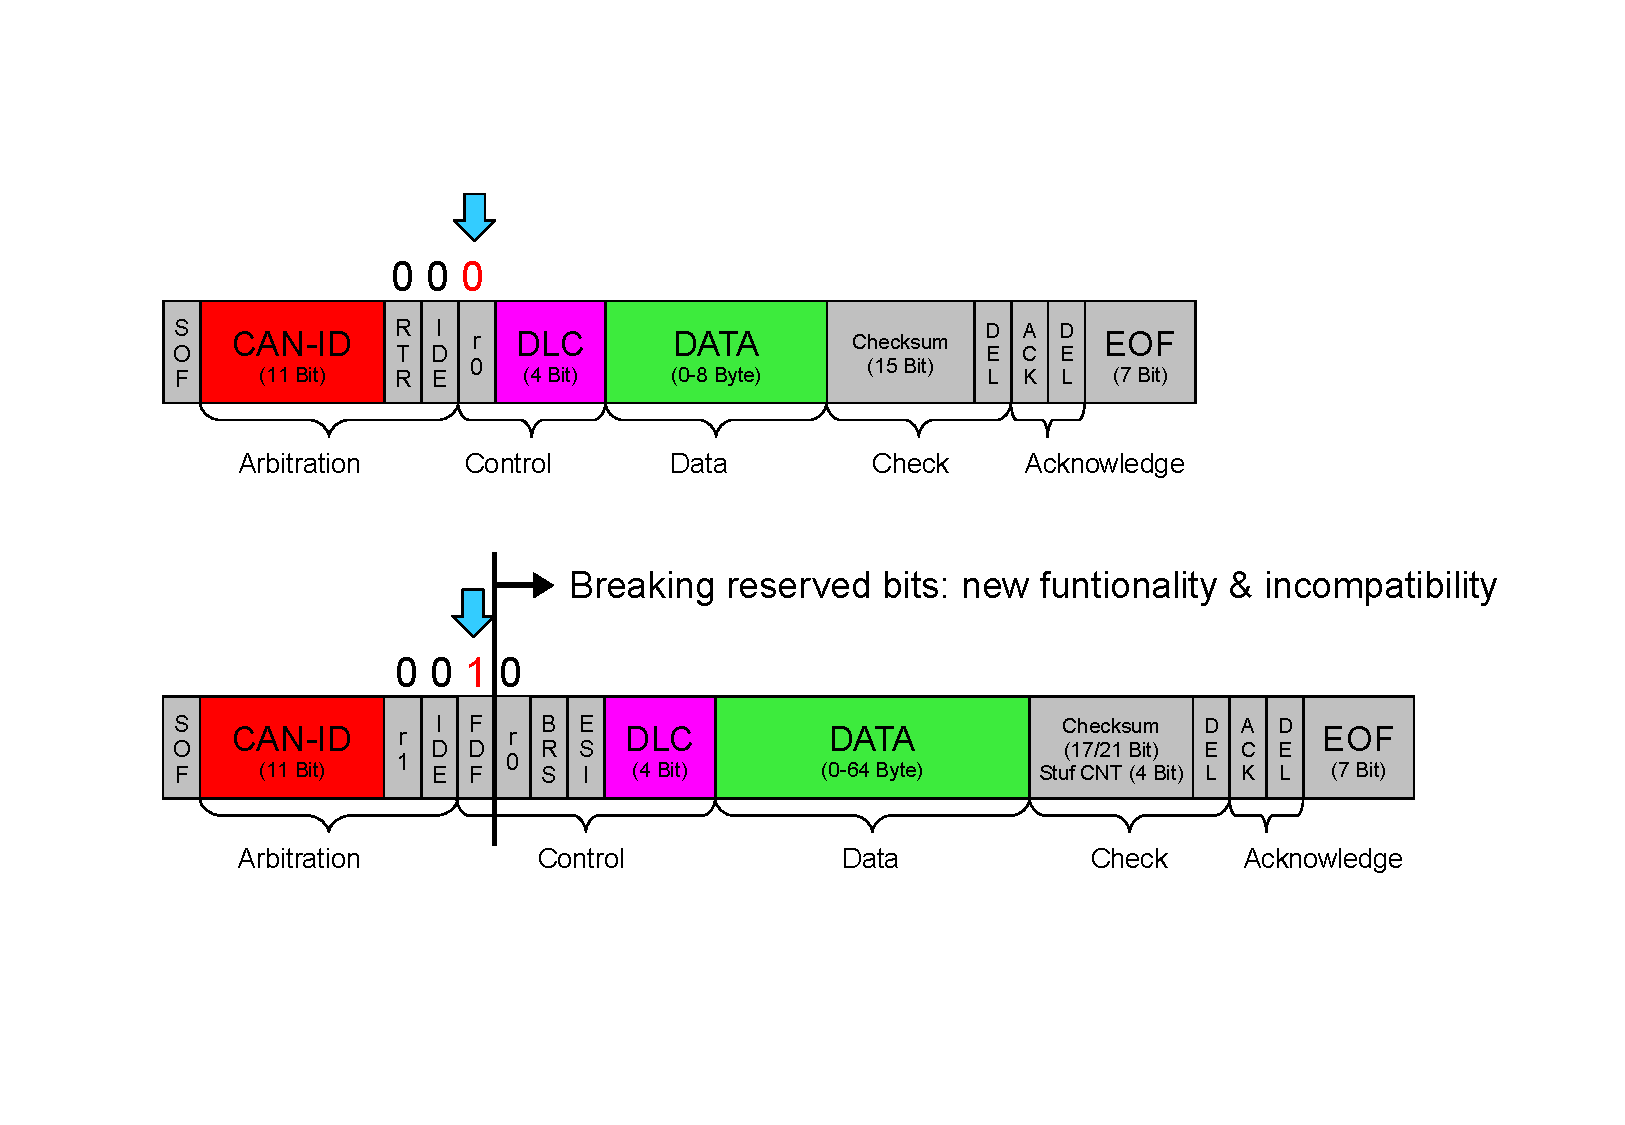
\includegraphics[width=1\textwidth]{agl2017-socketcan-can_fd}
  \caption{CAN and CAN FD difference \cite{canfd}}
  \label{fig:cancanfddifference}
  \end{figure}
  \subsection{Compatibility}
  \label{section:combability}
   There is no direct compatibility between CAN and CAN FD due to changes in the control field, see Figure ~\ref{fig:cancanfddifference}. Inconsistency appears in a reserved bit, which is always dominant 0 for CAN 2.0, but it now transforms into FDF flag indicating a CAN FD frame. Classic CAN 2.0 controller would not recognise CAN FD specific frames and would reject them while transmitting an error frame. Three new bits have been added into the control field. Reserved bit has been added for the possibility of future extension with a new protocol, BRS in recessive logic 1 indicates a faster bit rate shift of data phase and ESI informs about error passive - logic 1, or error active transmitter state.
   \subsubsection{Bit stuffing and CRC}
    The condition for bit stuffing has been changed. Stuffing bits can be added between SOF and newly at the end of the data field with the same principle as CAN 2.0. CRC now calculates with these stuff bits. Stuffed bits are also added in CRC, but with modified principle. CRC has been improved because several bits have been added and newly do not always have the same length. The checksum also includes stuff bit count to support CRC with data integrity.
   \subsubsection{Data length code mapping}
    One of the most significant differences is the DLC control field, which holds an individually coded length of the data. Data of arbitrary length of up to 64 bytes integrate into one of the possible intervals. First 8 bytes correspond to the standard CAN frame and continue with 12, 16, 20, 24, 32, 48 or 64 bytes length. This non-linear ordering stems from the historical reason that only 4 bits were available.
    \begin{figure}[H]
    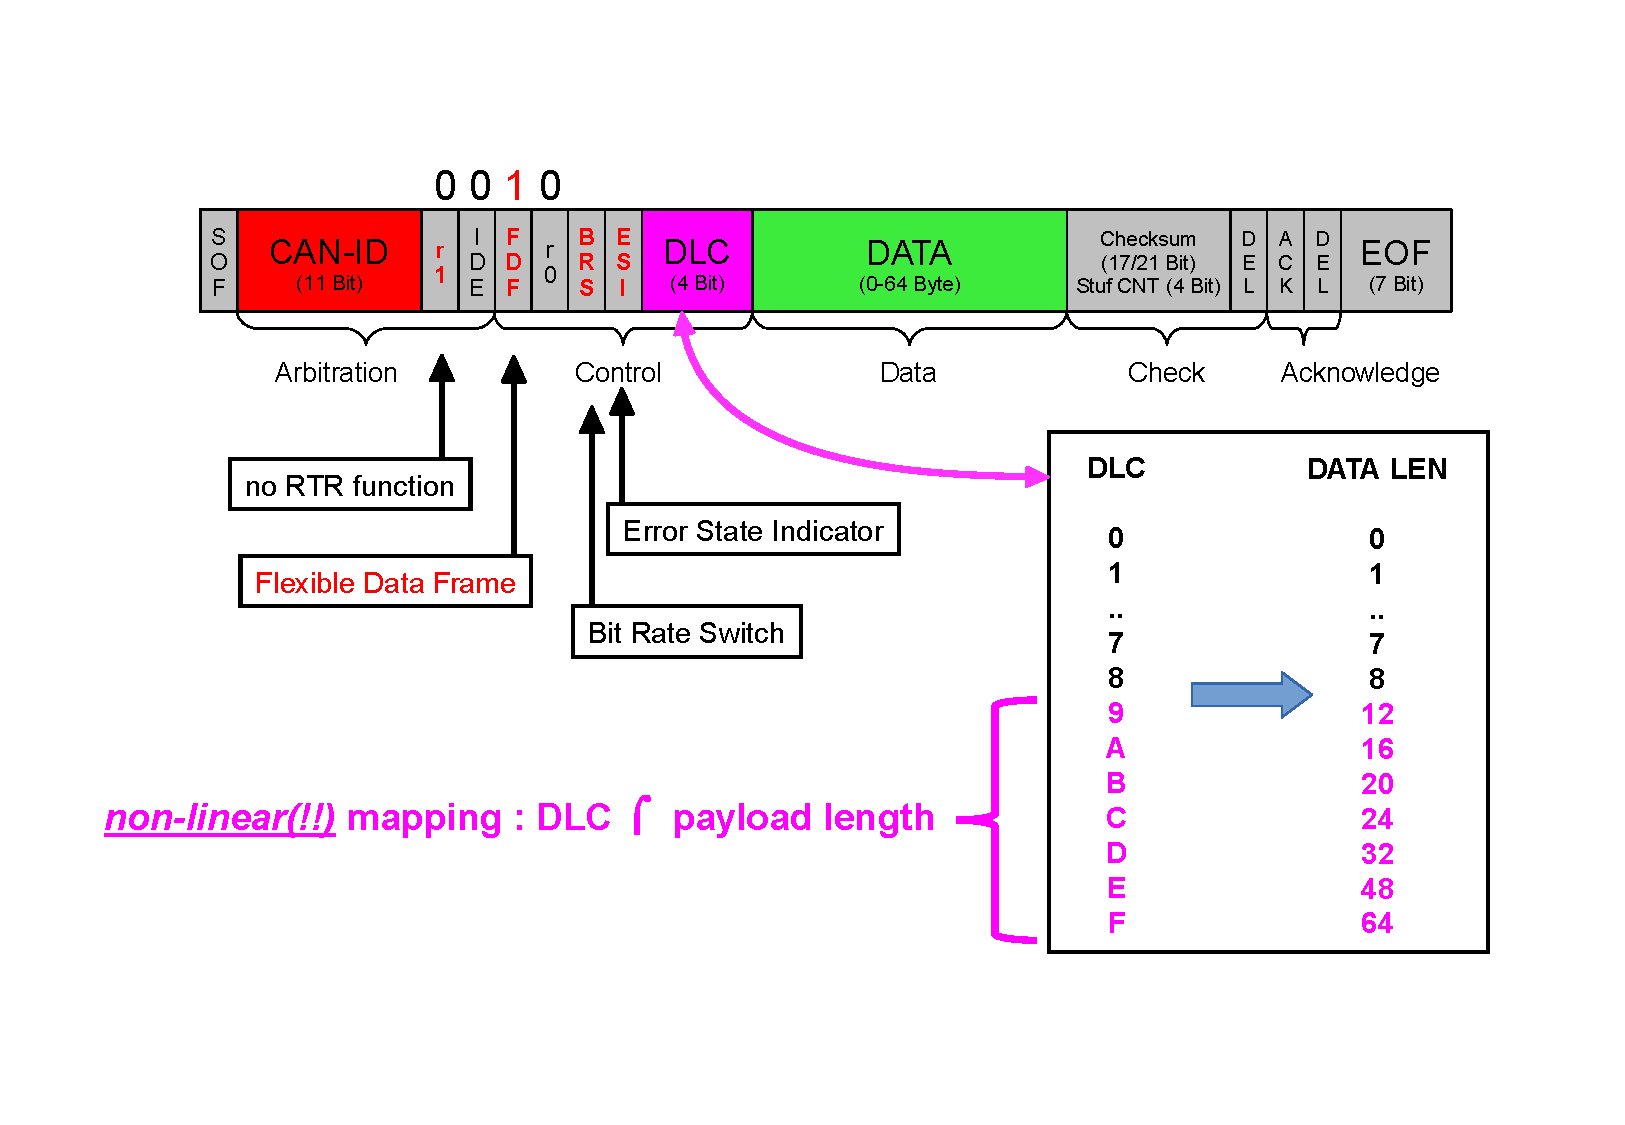
\includegraphics[width=1\textwidth]{agl2017-socketcan-can_fd_dlc}
    \caption{CAN FD frame DLC table \cite{canfd_dlc}}
    \end{figure}
 
\chapter{QEMU emulator}
 QEMU is a universal virtualisation tool as it is able to function in several distinctive modes. The original purpose was to launch a program compiled for another architecture as a user-space process without the need to change the current architecture (ARM, MIPS, Linux). However, it is used more frequently nowadays for a full system virtualisation including peripherals virtualisation. Support of the CAN bus and controllers emulation has already been accepted into the mainline. Nevertheless, the CAN bus standard  is evolving, and a new extended variant of the protocol was introduced in 2012. It is called CAN FD to highlight the use of higher bit rate for the data portion of the frame.

 \section{Automated testing}
 Linux is already able to handle CAN FD communication, even to create a virtual CAN bus and set up the communication there. A problem occurs with a new CAN interface driver development or implementation of a driver for another operating system. Most project maintainers want to be able to test new changes automatically, without all the hardware. It is one of the reasons why the integration of virtualisation of the CAN bus into QEMU started \cite{qemu_development}.

 \section{QEMU Object Model}
  The newest QEMU device model consists only of devices and properties\cite{qemu_qom}. Properties are the external interface to an object. That means it differs from the previous Qdev separation for devices and busses. New device creation is initialised with properties set to default values and with no parent. Each device has a unique name, derived from the parent name.

 \section{QEMU architecture}
  Linux mainlined Socket CAN API was selected as a connection between the host - real CAN hardware, and a guest system running QEMU with virtualised CAN devices. Each virtual CAN device is seen as a PCI device by the guest system. \\
  Two or more emulated controllers can be connected and create a virtual CAN bus, and this communication will be visible only in QEMU. One or more interfaces can be connected to the host system via SocketCan and will be observable in the host system through monitoring tools. However, it is necessary to connect only one controller to the host system. Otherwise, an infinite loop occurs. \\
  The image below serves as a quality description of emulation inside QEMU, and CAN support to QEMU emulator documentation provides a satisfactory explanation \cite[page 2-4]{qemu-mainline}.
  \begin{figure}[H]
  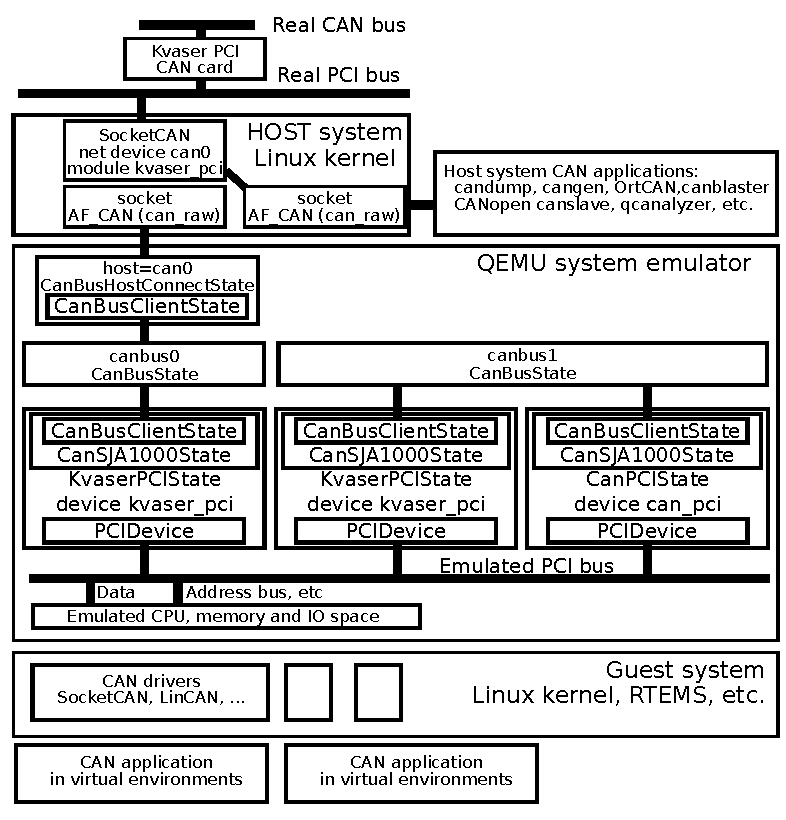
\includegraphics[width=1\textwidth]{qemu-can-bus}
  \caption{QEMU system emulator \cite{qemu-canbusexplain}}
  \end{figure}
 
 \section{QEMU CAN subsystem}
  To be able to access CAN bus in Linux, a physical card is required. Subsequently, a driver must be implemented, which understands the data sent over the bus. \\
  The emulated controller SJA1000 is I/O mapped to a single region of the emulated Kvaser PCI CAN card. Reading and writing to this region is directly mapped to the SJA1000 chip read or write operations, which supports only byte size access. \\
  QEMU also should be able to freeze, save the whole state into the prepared VmStateDescription structures and migrate to another computer, even to another architecture. \\

 \section{Coding style}
  QEMU coding style \cite{qemu-style} is similar to the recommended Linux kernel style.  The QEMU repository includes the script which checks the written code and displays all problems. The most common mistakes are tabs instead of 4 spaces, spaces or tabs on an empty line, incorrect use of parenthesis.
  \begin{verbatim}  ~/QEMU_PATH/scripts/checkpatch.pl ctucan_core.c\end{verbatim}
  The example above is a check script for correct code style of ctucan\_core.c.

 
\chapter{Implementation}
 The following part of this bachelor thesis consists of the implementation of CAN FD capable chip, which will support QEMU CAN subsystem. Essential required mechanisms have been implemented, such as transmission and reception.  
 \section{Integration}
  It is necessary to extend the QEMU side SocketCan interfacing because it accepts only CAN 2.0 messages. CAN FD support for SocketCAN has been accepted in the Linux kernel. Therefore, it is possible to be inspired there to expand the support of the CAN FD in the QEMU. When the bus enables frames of CAN FD standard, two following steps are necessary to happen. First, the SJA1000 chip emulation must be slightly modified to become CAN FD tolerant and not generate error frames. As the next part of CAN FD integration, a CTU CAN FD PCI card based on the Kvaser PCI CAN card emulation implemented by Jin Yang and Pavel Pisa has to be added. Last implementation goal is an emulation of a CTU CAN FD IP core as the controller mapped into the CTU CAN FD PCI card.
  
 \subsection{SocketCan support for CAN FD}
  Initial host SocketCan support has been added for CAN FD. SocketCan subsystem, allows sending and receiving from the CAN 2.0 controller. CAN FD frames handling requires to send structure with a different memory size to the SocketCan socket determined by the file handle. Structure qemu\_can\_frame has been extended to hold to provide space for up to 64 data bytes. Furthermore, a property called flags has been added into the message structure. The flags property is uint8\_t and holds additional bits newly defined in the standard such as BRS, ESI and FDF, see~\ref{section:combability}. DLC property remains identical, but the CAN frame stores actual data bytes count instead of DLC code because it simplifies the kernel's back-checking for record lengths.

 \subsection{CTU CAN FD core support}
  Initial CTU CAN FD core support was started as a copy of SJA1000 controller emulation, which was the sole supported controller at the time of the project launch. The creation of CTU controller supporting CAN FD  has already commenced. \\
  When CTU CAN is integrated into a PCI Express board, then two BARs (Base Address Regions) are expected by the driver. The first one stores value to identify the CAN core and provides a number of integrated core instances in the other region. The first region is read-only and is accessed by ctucan\_pci\_id\_cra\_io\_read function. The second region maps registers of the core instances one after another. As an I/O mapped region, it can be accessed by reading ctucan\_pci\_cores\_io\_read function, which immediately calls core function ctucan\_mem\_read with a correctly aligned memory address as the parameter. Function ctucan\_pci\_cores\_io\_write operates on the same principle as the read function. The registers to control PCI Express MSI (Message Signaling Interrupts) and other FPGA chip-specific control functions are also mapped at a certain offset to the first region. At the beginning of my work, attention is focused on the critical registers for transmission and reception. Apart from the control registers, correct behaviour of access for four TX buffer and cyclic FIFO RX buffer must be also implemented in the first stage. Subsequently, less important read/write registers are implemented, for example traffic counters or controller state diagnostics.
 
 \subsection{Registers emulation}
  CTU CAN FD core register definitions are generated from IPXACT CTU CAN core specification (version 2.1), which is a part of the IP core design architected by Ing. Ondrej Ille. It is a significant amount of memory mapping structures, more specifically unions, which define the layout of bits in registers in real hardware. It distinguishes between several types of bits in hardware registers, read-only, write-only, and read/write bits. Everything is included in product documentation, and it is necessary to follow it precisely for correct emulation behaviour. The documentation describes the functional description of CTU CAN FD, programmers model, and parameters of CTU CAN FD. In order to ensure core emulation which works with Linux kernel driver, each bit has to be handled according to the specification. Accessing CTU CAN FD device data is possible only through the individual registers, meaning memory access is aligned with words. To be able to read or write, it is necessary to call a read or write function with the correct address of the required register as a parameter. \\
  Control registers have several functionalities; write-only commands to change inner state, status information about internal traffic counters, errors report, etc., and reading of received data.
 
  \subsubsection{Data structures}
  The internal state of CTU CAN FD controller must be stored in some data structure in QEMU software model. CTU CAN FD core register definitions enable to create variables, which are structured in the same way as bits of a specific register in VHDL design. It is not necessary to create a variable for each register. Some control registers are write-only, for sample command control registers, which changing inner state, but it is not a necessity to store them. These data structures are defined in ctucan\_core.h and, together with Tx and Rx buffers and auxiliary variables form and hold the whole CTU CAN FD core state. \\
  CTU CAN FD PCI is described and registered in a fundamental structure TypeInfo ctucan\_pci\_info. Every single device in QEMU device tree must have one. It contains a name, as TYPE\_CAN\_PCI\_DEV, a parent in the hierarchal based tree; as for PCI device, it is TYPE\_PCI\_DEVICE, pointers to initialisation function and some further additional information. CTU CAN FD core is written generically, which means that it is stand-alone and it is not unconditionally a part of the PCI device. CTU CAN FD PCI has a place for two core slots when PCI device ctucan\_pci\_instance\_init function is processed; therefore, two instances of CTU CAN FD core are created, and each takes place in one slot. PCI has one more initialisation function ctucan\_pci\_class\_init where are realise and exit function sets and other information about PCI device relevant for the system. 
Each device in the QEMU should be able to store the whole state into VMStateDescription structures and be able to run from this state after some break again. This state storing is hierarchically based. CTU CAN FD PCI device is no exception among others device, VMStateDesciption structure called vmstate\_ctucan\_pci is defined in ctucan\_pci.c and stores PCI DEVICE state.
   \begin{verbatim}   VMSTATE_PCI_DEVICE(dev, CtuCanPCIState),
   VMSTATE_STRUCT(ctucan_state[0], CtuCanPCIState, 0,
                   vmstate_ctucan, CtuCanCoreState)\end{verbatim}
  Therefore, both CTU CAN FD core states are stored, the structure where they are stored is called vmstate\_ctucan and is defined in ctucan\_core.c. There are again direction, how to store entire CTU CAN FD core state. This time with basic variable types such as
   \begin{verbatim}   VMSTATE_UINT32(mode_settings.u32, CtuCanCoreState)\end{verbatim}
  VMStateDescription should also store the Rx and Tx buffers.
  \begin{verbatim}   VMSTATE_BUFFER(rx_buff, CtuCanCoreState)\end{verbatim}
 
 \subsection{Interrupts}
 Interrupts are called to inform the CPU about finished processing of command or other hardware state change which needs the CPU intervention. For a sample, inform the CPU that the transmission has ended. Another example is a reception and the need to inform that the data are waiting in Rx FIFO. Several conditions must be met and the corresponding interrupt status set to 1, and then it is possible to fire an interrupt.
  \begin{verbatim}qemu_irq_raise(s->irq);\end{verbatim}
  It is possible that certain interrupts are not enabled or has been processed by the software, then the function 
  \begin{verbatim}qemu_irq_lower(s->irq);\end{verbatim}
  is called.
 
  \subsubsection{Interrupt mask}
  Interrupt mask could be arbitrarily set. After power-up or reset, the interrupt mask is full of zeros, meaning that all interrupts are enabled. When the corresponding interrupt is required, the corresponding interrupt mask bit has to be zero; when this condition is met, an IRQ can be fired.
  
  \subsubsection{Invoke interrupt}
  The picture below demonstrates the conditions for the interrupt to be fired. First, it must be 0 (unmasked) in the interrupt mask. Another condition is that the interrupt must be enabled. CTU CAN FD core sets the interrupt status bit to 1 when conditions for the interrupt are fulfilled; for example, a frame is received from the bus. In such a case, the interrupt would be invoked by calling function 
  \begin{verbatim}qemu_irq_raise(s->irq);\end{verbatim}
  \begin{figure}[H]
  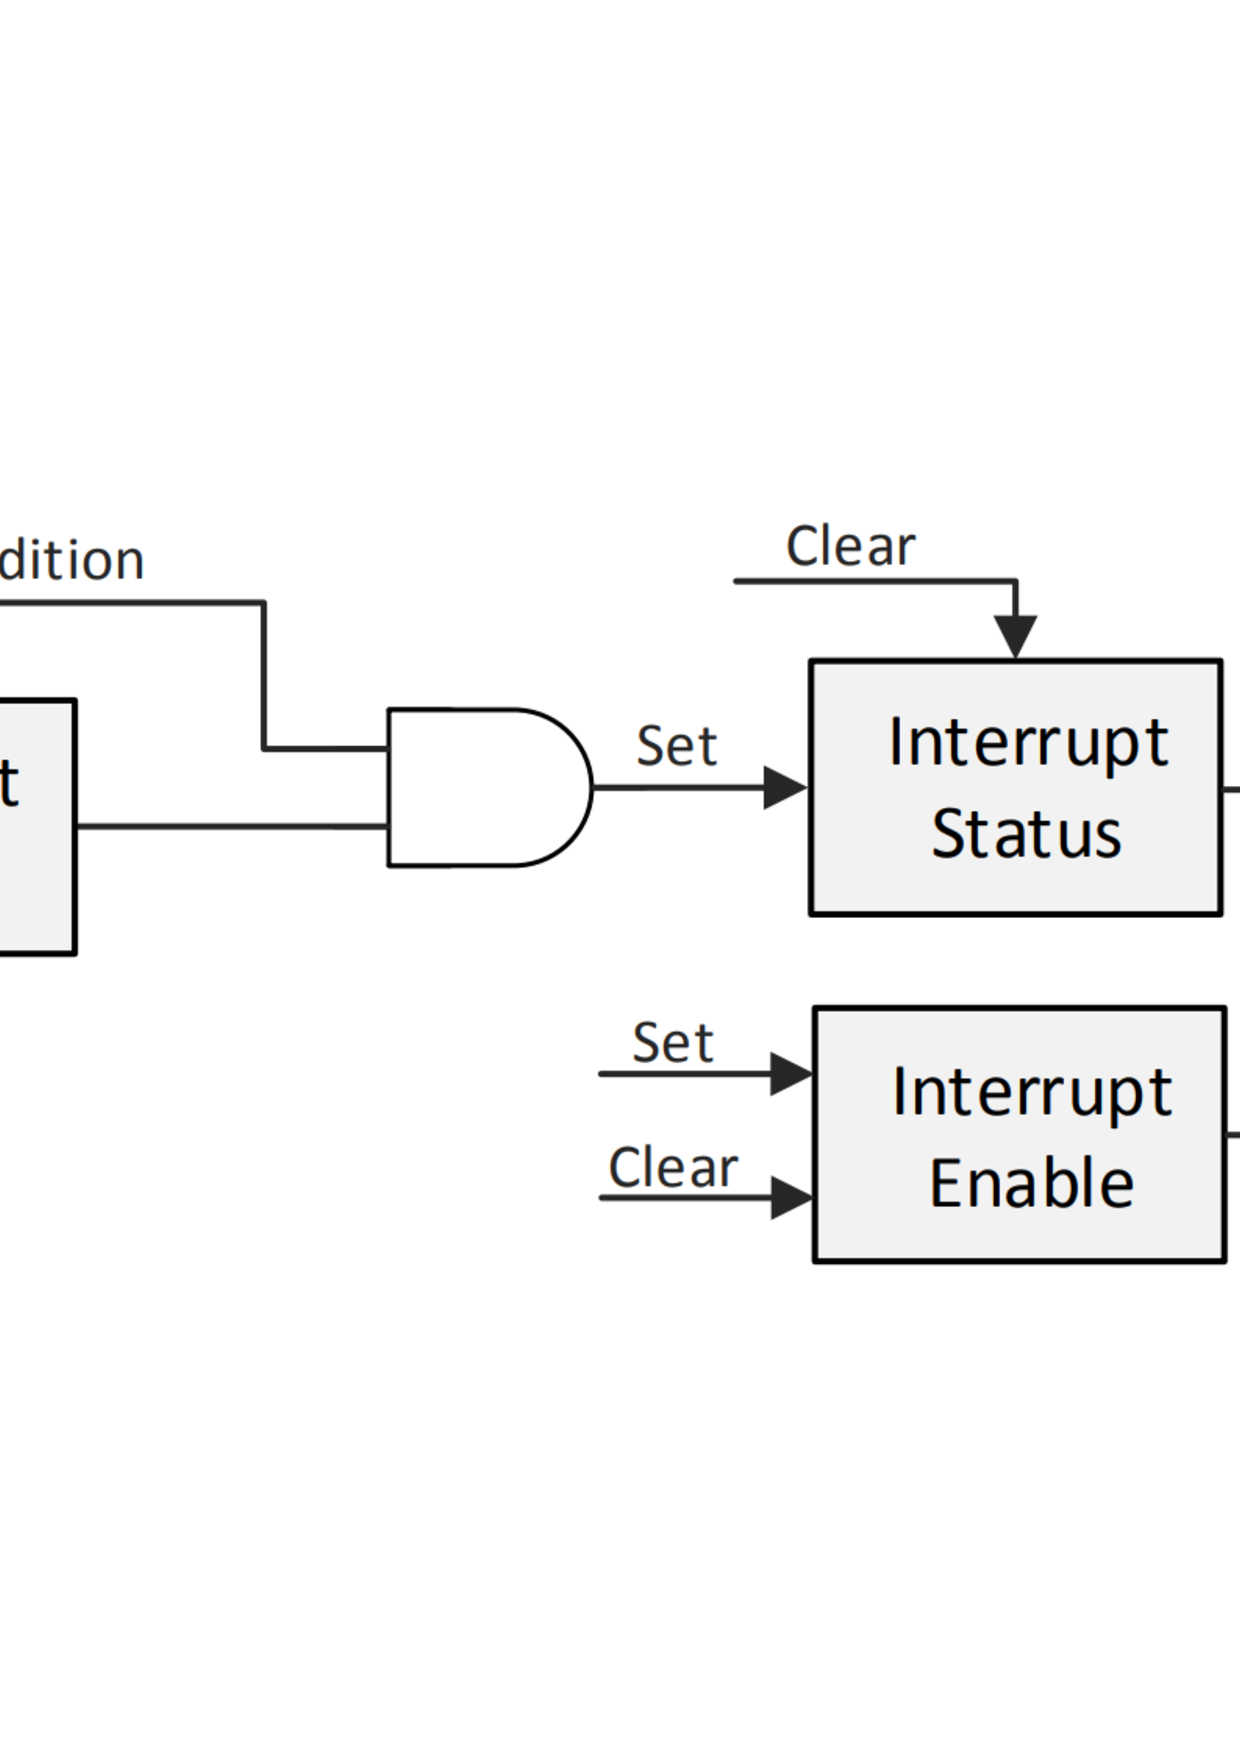
\includegraphics[width=1\textwidth]{progdum-interrupts.pdf}
  \caption{Interrupts \cite{progdum}}
  \end{figure}
 
 \subsection{SJA1000 CAN FD tolerant}
 Emulated chip SJA1000 would not be able to communicate on the bus where CAN FD frames are sent without a few changes. First, Using new flags as BRS and ESI should be avoided. At the minimum, FDF and BRS bits must always be set to 0 during transmission. Another problem is posed by frames which hold more than 8 bytes of data. If the controller tries to receive this frame, it can lead to undefined behaviour. Therefore, each message with the data phase longer than 8 bytes must be ignored. These changes are sufficient to create CAN FD tolerant SJA1000 emulated chip. It corresponds now with the design of OpenCores SJA-1000 FD Tol. OpenCores SJA-1000 controller modified to ignore CAN FD frames which allows it to coexists and send frames on the network with CAN FD traffic. The core is packed as a Xilinx Vivado component \cite{sja1000-fdtol}.

 \section{Transmission}
  TX buffers are used for transmission by CTU CAN FD. They are filled with software, for example a Linux kernel driver, which knows the mapping of TX buffers and stores the whole frame word after word. When the whole frame is stored into an arbitrary Tx buffer, Tx command TXCR is set. During the processing of TXCR command, i.e. writing to an exact register, the controller sets the buffer into the READY state and immediately sends the frame and changes buffer state into buffer OK state. There is no implementation of delay yet. It follows that the transmission cannot be aborted. During this procedure, all Tx buffers are iterated, and Tx buffer in the READY state, which corresponds to the flag of the related buffer, is sent.

 \subsection{TX buffers}
  The initial implementation of TX buffers is 0x50 bytes uint\_8t array, computed to be at the minimal level of sufficiency of CAN FD frame. Four Tx buffers are in CTU CAN FD prepared for the transmission. Support of transmission buffers is necessary for correct message sending. Buffer with a stored whole frame inside is transmitted to the bus. The controller then informs the CPU through interrupt requests that transmission transpired and that at least one buffer is again in OK state.

  \subsubsection{Buffer states}
  The initial state for all four buffers is the EMPTY state. It indicates that a buffer available to use. The OK state, which is set after successful transmission, has an identical meaning. When the data are ready to be sent, it corresponds to the READY state. The ABORT state is not implemented due to no transmission delay, and the same applies for the FAILED state. The FAILED state occurs when several unsuccessful attempts are made.
 
 \subsection{Commands}
  Several Tx commands are defined. TXCE is able to reset buffer state to initial state. This command could restore the FAILED state buffer back to functionality, also affects the OK state and the ABORTED state. TXCA changes the READY state into the ABORTED state. Theoretically, it is possible, but transmission delay is not implemented, so it is not possible to reach this command functionality. The most important command TXCR sends a frame to the bus. Simultaneously set the OK state, the FAILED state or the EMPTY state to the READY state.
 
 \subsection{Buffer to frame}
  Before sending any data to the bus, it is necessary to move them from an internal stored buffer - this format is defined the same way as the CTU CAN FD core register definitions - to a generally understandable SocketCan frame format. The first step is the initialisation of QEMU CAN frame structure, and data are loaded from the internal buffer by mapping unions which enable to copy the correct bits. At the end of the process, it is possible to directly memcopy the data phase. Every frame stored in Tx buffer is stored there according to the same rules, so header has always 16 bytes and the maximum of the data phase can be 64 bytes.
  \begin{verbatim}memcpy(frame->data, buff + 0x10, 0x40);\end{verbatim}
 
  \subsubsection{Ambiguous problems}
   Real bytes count is encoded by the CAN FD standard into DLC. It is necessary to take care of this non-linear mapping because in the internal buffer, DLC is stored by CAN FD standard; however, it is required to hold in DLC real bytes count in the frame which would be sent to the bus because it simplifies the kernel's back-checking for record lengths. Non-linear mapping solution can be found in can\_emu.h as dlc2len function. The identifier poses a minor problem as it exists as one number in the frame, but it is divided into the base and the extended identifier in defined internal buffer layout. The solution is simple, in case of using the only base identifier, the base identifier is assigned to CAN ID. In the opposite case, the extended identifier is assigned first, with the subsequent use of logical OR to add the base identifier shifted by 18 to the left. 
   
 \section{Reception}
  Reception is implemented through a single FIFO organised Rx buffer. All incoming frames from the bus are stored in a successive order. Reading from Rx buffer is processed by the RX\_DATA register. CTU CAN FD is able to recognise the first and the last words of the frame in the Rx buffer. When the whole frame is read by software, it can continue with the next frame reading immediately.

 \subsection{RX buffer}
  Rx buffer is uint\_8t array with an arbitrary length. After each reception, RXFRC is updated. Several messages can be stored during the usual system running, resulting in the need to determine frame boundaries during words reading by SW. This is the reason why the byte remainder counter was added to the core state. After verifying that the Rx buffer is not empty, the CAN frame reminder appears as an essential element during RX\_DATA register reading. If the CAN remainder is zero, we read the first word of the new frame. Through frame alignment definition, it is possible to map the correct structure on this word and read RWCNT from which the length of the frame is calculated. Rx buffer overrun occurs when the traffic incoming from the bus fills up Rx FIFO and reading and processing of the messages by the guest driver is too slow. At the moment when the new frame cannot be stored, the overrun interrupt is invoked, and the frame is discarded. It is possible to flush the Rx buffer by writing logic 1 to the control register COMMAND flag RRB. 
 
  \subsubsection{FIFO implementation}
   There are several possibilities of how a FIFO could be implemented. For data reading per bytes, a tail pointer is used very frequently. Head pointer is also essential but is used only for storing the whole frame. Instead of the head pointer, it was decided to store accurate bytes count in the Rx buffer, from which it is easy to calculate the head pointer. Actual bytes count is used in several conditions across the CTU CAN FD.
 
 \subsection{Frame to buffer}
  Before it is possible to store the incoming frame into the Rx buffer, it is necessary to convert the frame from a generally understandable SocketCan frame format to an internal stored buffer - this format is defined in the same way as the CTU CAN FD core register definitions. For this purpose, the TMP buffer is created with the size of one CAN FD frame. This buffer must be set to zeros by memset.
  \begin{verbatim}memset(buff, 0, CTUCAN_MSG_MAX_LEN * sizeof(*buff));\end{verbatim}
  The data are loaded from the frame to the internal TMP buffer by mapping unions which enable to copied bits to the correct place in the TMP buffer. The data phase can be copy directly by memcpy.
  \begin{verbatim}memcpy(buff + 0x10, frame->data, 0x40);\end{verbatim}
 
  \subsubsection{Ambiguous problems}
   They bear a high similarity to transmissions problems, but one change arises in this case. There is an urgency to count bytes in the frame correctly because it is used later for copying from a TMP buffer into the Rx buffer. Fortunately, the non-data phase always has 16 bytes. The frame holds DLC in the exact bytes count; we can therefore use this number, but on one condition - the resulting number of bytes must be aligned with words.
   \begin{verbatim}   bytes_cnt = (bytes_cnt + 3) & ~3;\end{verbatim}
   CAN ID is stored in the frame as a singular number. Internally, it is necessary to divide it into the base and the extended identifier. In the case of the base identifier only, the first 11 bits should use logical AND with 0x3FF. When the extended identifier with 29 bits is used, it is divided into the 11 bits identifier base and the 18 bits extended identifier. First, CAN ID must be masked by logical AND with 0x3FFFF and stored to the extended ID. In the following step, CAN ID must be shifted to the left by 18 and masked by logical AND with 0x01FFFC0000.
  
 \section{Hardware Reset}
  A hardware reset is called in two cases; always after a CTU CAN FD power-up, or it can be called through writing logic 1 to the control register MODE flag RST. Following a power-up, the reset is more likely used to set up correct reset values. A more complicated situation occurs during a reset in the middle of work. In addition to setting the reset values, the work in progress must be cleaned up by resetting traffic counters, status control registers and interrupts. Each Tx buffer should return into the empty state. It is also necessary to flush the Rx buffer. It involves several steps - resetting tail position pointer, buffer bytes count and, in case of reset during frame reception, also the frame reminder.
 
\chapter{Testing}
 The chapter focuses on the set of commands necessary to prepare the testing environment and verify the functionality of written code, specifically if the data pass through and message identifications correspond.

 \section{Actual testing environment setup}
  This section describes the setup which was used. This bachelor project was developed in a system with Windows 10 where it runs utility for virtual machines VMware Workstation 15 player in its free version available for non-commercial use only \cite{vmware}. \\
  Virtual machine Ubuntu 18.04.3 LTS \cite{ubuntu} runs on VMware. The entire work with QEMU takes place inside the Ubuntu. QEMU also uses virtualisation, so during the work, for testing purposes, the next Linux system emulates inside the QEMU and results in virtualisation chain, which is not the best practice for working, but fortunately, it is possible. In this case, QEMU uses the same build of the Linux kernel as an external system. It was kernel version 5.3.0-51-generic for Ubuntu 18.04.3 LTS at the time of the writing of the thesis. QEMU can be run with
  \begin{verbatim}   -nographic\end{verbatim}
   parameter, and then it uses the current terminal window as its native console.
   \begin{verbatim}   -append "console=ttyS0"\end{verbatim}
This parameter commands Linux kernel to use ttyS0 as the system console output for error and informative messages which are directed to the terminal window from which they can be easily copy-pasted and saved for future analysis. To quit QEMU running in the console, a  non-trivial key combination is required, specifically Control + 'a'  'x'. A problem occurs several times after the Ubuntu software update. The kernel version is precisely set, so it must be updated.
  \begin{verbatim}-kernel   /boot/vmlinuz-5.3.0-46-generic\end{verbatim}
  The RAM disk needs to be generated
  \begin{verbatim}   mkramdisk-mf624\end{verbatim}
  and then needs to be added as a Qemu parameter 
  \begin{verbatim}   -initrd ramdisk.cpio\end{verbatim}
  Before starting the QEMU, it is possible to set a shared directory which could be used for data transfer between host and guest systems during QEMU's run. This allows the option to add files or binaries into the emulated system during its run. In this example case, a sharreddir directory (in the same directory as a Qemu launcher qemu-run) is mapped with the use of p9 protocol to simple QEMU virtual file system by the QEMU parameter below.
 \begin{verbatim}-virtfs local,path=shareddir,security_model=none,mount_tag=shareddir\end{verbatim}
 These code snippets bellow are paths to access to directories for communication between inner and outer Linux systems during QEMU emulation. A file from the host system then can be stored to
  \begin{verbatim}   ls ~/QEMU_RUN_DIR/shareddir\end{verbatim}
  and will be visible from the guest system in
 \begin{verbatim}   ls mnt/shareddir/bin/\end{verbatim}
 \section{Test SW}
 This is a user-space program for communication in the bus testing. It can be found in the public git repository CTU CAN FD IP core  \cite{driver-repo} ctucanfd\_ip\_core/driver, it must be generated by the Makefile. The Makefile generates program called test, and then it is sufficient to copy it to the shared directory.
 \begin{verbatim}   test-ctucan -p -T -I 0x123 -f -b
          [-p] search core through PCI card
          [-T] periodically transmit
          [-I] set the identifier
          [-f] transmit CAN FD frames
          [-b] bitrate switch
          [-i] use instance 0 or 1 from certain PCI card\end{verbatim}
 PCI must be enabled before this user-space program is launched, but at the same time driver can not be loaded. \\
 To enable CTU CAN FD PCI device
\begin{verbatim}   lspci -n -d 1760:ff00\end{verbatim}
is used to find on which PCI bus and in which "socket" the card is present and then to use for example.
\begin{verbatim}   echo 1 >/sys/devices/pci0000:00/0000:00:06.0/enable\end{verbatim}
where bus number and device slot is adjusted according to lspci output.\\
 It is beneficial for debugging to have the user-space program.
 
 \section{Driver}
 The driver module must be loaded to the Linux kernel and communication set up.
 \begin{verbatim}  modprobe ctucanfd_pci
  ip link set can1 type can bitrate 1000000 dbitrate 1000000 fd on
  ip link set can1 up
  cangen can1 -f\end{verbatim}
 Sequence for testing purpose. Load CTU CAN FD module into the Linux kernel, set up a virtual CAN interface and run random CAN FD frames generator.\\
 SocketCan offers several userspace utilities and tools. The following two tools are enough for basic testing.
 \begin{verbatim}  candump [can0]
  cangen  [can0]
          [-f] CAN FD frames
          [-g] time frequency in ms\end{verbatim}
 Necessary tools to display, record, generate and test CAN traffic \cite{can-utils}.

 
\chapter{Conclusion}
 The goal of this thesis was to analyse the differences between CAN 2.0 and CAN FD standards and to describe QEMU CAN subsystem, and to use this knowledge in the subsequent part and create a functional emulation of a CAN FD communication bus and model of a CAN FD capable controller. Both targets were achieved.This thesis could be found in git repository \cite{thesis-repo}.

 \section{Work already completed}
  This project analyses the basic QEMU concept and how to work with it as a full system emulator. It also demonstrates a proper coding style for QEMU. The next part analyses CAN frames differences between standards to be able to understand which parts changed and how to implement them. It is necessary to know the role of each bit of CAN frame to be able to operate with them. The analysis offers a group of often-used commands which help with the workflow and with the testing.
 
 \subsection{Transmission and reception}
  Emulation of CAN FD communication was achieved. QEMU virtual CAN bus now supports CAN FD frames and preservers the possibility of CAN 2.0 communication only. Due to the changes in the bus frame, a stand-alone chip SJA1000 was improved to make it CAN FD tolerant. Furthermore, it can behave as an active device during communication under the condition of ignoring frames with data phase longer than 8 bytes. Several testing methods proved the correct transmission.

 \section{Implementation}
  An already functional emulation of CAN bus and stand-alone SJA1000 controller support has been extended, CAN FD support has been added, and  CTU CAN FD core controller is now available with modified card CTUCAN PCI. Nowadays, the transmission of CAN FD frames is available. The new implementation preserves the previous functionality of sending CAN 2.0 frames.

 \subsection{Future implementation goals}
  It is possible, consider message rate slowdown as on a real CAN bus. Some mechanism prevents loss of messages to a certain level when a guest application is slow. We can convert CAN bus model from plain C to QOM (Controllers are QOM/Qdev already). We can add more CAN controllers model emulation (BOSCH/Ti C CAN, Freescale FlexCAN, etc.).
 
 \subsection{Transmission delay}
 To achieve the goal of behaving like real hardware, some delay can  be implemented between the command to send data from the buffer and the real sending data on the bus. Because of this delay, a possibility emerges to abort transmission before it is sent.
 
 \subsection{TXT buffer selection}
  In the actual state of implementation, buffer selection does not take any place. Buffer selection should be implemented together with transmission delay because all four buffers are every time, when TXCR is set, iterated and the Tx buffer in the READY state, which corresponds to the flag of the related buffer are data immediately transmitted.
 
 
\renewcommand\bibname{References}
\begin{thebibliography}{1}
\bibitem{qemu-mainline} Pavel Pisa, Jin Yang, Michal Sojka, QEMU CAN Controller Emulation with Connection to a Host
System CAN Bus, http://rtime.felk.cvut.cz/publications/public/rtlws2015-qemu-can.pdf, accessed: 2020-05-20.
\bibitem{ctu-canfd-core} CTU CAN FD IP Core, https://gitlab.fel.cvut.cz/canbus/ctucanfd\_ip\_core, accessed: 2020-05-10
\bibitem{canfd_calculator} CSS Electronics, CAN FD EXPLAINED - A SIMPLE INTRO: Efficiency and Avarage Bit Rates, https://docs.google.com/spreadsheets/d/\\16XIceuoG\_YBlgyFKXxjYQk2016ln3NeEC68yoMFvwkA/edit\#gid=0, accessed: 2020-05-17.
\bibitem{ctu-canfd} Martin Jeřábek, Open-source and Open-hardware CAN FD Protocol Support, https://dspace.cvut.cz/bitstream/handle/10467/80366/F3-DP-2019-Jerabek-Martin-Jerabek-thesis-2019-canfd.pdf, accessed: 2020-05-17.
\bibitem{ctu-project} pcie-ctu\_can\_fd, https://gitlab.fel.cvut.cz/canbus/pcie-ctu\_can\_fd, accessed: 2020-05-17.
\bibitem{progdum} Czech Technical University in Prague, Faculty of Electrical Engineering, Department of Measurement, CTU CAN FD IP CORE Datasheet, http://canbus.pages.fel.cvut.cz/ctucanfd\_ip\_core/Progdokum.pdf, accessed: 2020-05-19
\bibitem{ECUs} CSS Electronics, CAN BUS EXPLAINED - A SIMPLE INTRO (2020), https://www.csselectronics.com/screen/page/simple-intro-to-can-bus/language/en, accessed: 2020-05-16.
\bibitem{can_frame} Complete CAN Frame, https://upload.wikimedia.org/wikipedia/commons/5/5e/CAN-Bus-frame\_in\_base\_format\_without\_stuffbits.svg, accessed: 2020-01-16.
\bibitem{can_Vd} Texas Instruments, Automotive Controller Area Network (CAN) Overview and Training, https://www.youtube.com/watch?v=YrJn2AyWVBc - time 4:40, accessed: 2020-05-16.
\bibitem{can_crc} Vector E-Learning, Introduction to CAN (EN), https://elearning.vector.com/mod/page/view.php?id=370, accessed: 2020-05-16.
\bibitem{priority_can} CSS Electronics, CAN FD EXPLAINED - A SIMPLE INTRO (2020), https://www.csselectronics.com/screen/page/can-fd-flexible-data-rate-intro, accessed: 2020-05-17.
\bibitem{canfd} Oliver Hartkopp, The CAN Subsystem of the Linux Kernel, https://wiki.automotivelinux.org/\_media/agl-distro/agl2017-socketcan-print.pdf by Oliver Hartkopp - page 49, accessed: 2020-04-01.

\bibitem{canfd_dlc} Oliver Hartkopp, The CAN Subsystem of the Linux Kernel, https://wiki.automotivelinux.org/\_media/agl-distro/agl2017-socketcan-print.pdf by Oliver Hartkopp - page 50, accessed: 2020-04-01.
\bibitem{qemu_development} RTEMS, QEMU with CAN Emulation, https://devel.rtems.org/wiki/Developer/Simulators/QEMU/CANEmulation, accessed: 2020-05-18.
\bibitem{qemu_qom} QEMU, Features/QOM, https://wiki.qemu.org/Features/QOM, accessed: 2020-05-18.
\bibitem{qemu} QEMU, What is QEMU, https://www.qemu.org/, accessed: 2020-01-18.
\bibitem{vmware} VMware, Workstation 15, Playerhttps://www.vmware.com/products/workstation-player/workstation-player-evaluation.html, accessed: 2020-01-18.
\bibitem{ubuntu} Ununtu, Download Ubuntu Desktop, https://ubuntu.com/download/desktop, accessed: 2020-01-18.
\bibitem{sja1000-fdtol} sja1000-fdtol, https://gitlab.fel.cvut.cz/canbus/zynq/sja1000-fdtol, accessed: 2020-05-20.
\bibitem{qemu-canbusexplain} Pavel Pisa, GNU/Linux, CAN and CANopen in Real-time Control Applications, https://www.linuxdays.cz/2017/video/Pavel\_Pisa-CAN\_canopen.pdf, accessed: 2020-01-20.
\bibitem{qemu-style} qemu/CODING\_STYLE, https://github.com/portante/qemu/blob/master/CODING\_STYLE, accessed: 2020-01-20.
\bibitem{driver-repo} ctucanfd\_ip\_core driver, https://gitlab.fel.cvut.cz/canbus/ctucanfd\_ip\_core/-/tree/master/driver, accessed: 2020-05-17.
\bibitem{linux-style} The Linux Kernel, Linux kernel coding style, https://www.kernel.org/doc/html/v4.10/process/coding-style.html, accessed: 2020-05-17.
\bibitem{mc} MC, Welcome to the Midnight Commander Development Center, https://midnight-commander.org/, accessed: 2020-01-17.
\bibitem{rdwrmem} Pavel Pisa, Simple program to dump and write physical or device provided
  memory locations from Linux userspace, http://cmp.felk.cvut.cz/~pisa/linux/rdwrmem.c, accessed: 2020-01-17.
\bibitem{can-utils} linux-can/can-utils, Linux-CAN / SocketCAN user space applications, https://github.com/linux-can/can-utils/, accessed: 2020-01-17.
\bibitem{thesis-repo} charvj/ctucanfd-thesis https://github.com/charvj/ctucanfd-thesis/tree/master, accessed: 2020-05-22.
\bibitem{project-doc} ctucanfd\_emulation, https://gitlab.fel.cvut.cz/canbus/qemu-canbus/-/wikis/ctucanfd\_emulation
\end{thebibliography}
 
\appendix
\chapter{Installation guide for programmers}
  Check installation of git versioning system by
  \begin{verbatim}  git --version\end{verbatim}
  if there is no installation on computer write command
  \begin{verbatim}  sudo apt install git\end{verbatim}
  Now pull QEMU mainline from git
 \begin{verbatim}  git clone git://git.qemu.org/qemu.git\end{verbatim}
  Will continue with proper installation way. \\
  Until the project is not in mainline, it could be found here.
  \begin{verbatim}   git remote add gitlab-fel https://gitlab.fel.cvut.cz/canbus/qemu-canbus.git
   git fetch --all
   git checkout -b charvj10-canfd gitlab-fel/charvj10-canfd\end{verbatim}
   For more information, see the project's documentation page \cite{project-doc}.

\chapter{Useful commands}
  It is useful to know debugging tools and other utilities available in the system to proceed with the work. It could make progress faster and simpler. The shortlist of advice tools means  which were used during this project development follows.
 \section{Linux}
  For experienced GNU/Linux users, the following commands are natural, but for users-beginners, or predominantly Windows programmers, they might be helpful. The advice also contains shortcuts for Midnight Commander \cite{mc}. MC during the bachelor project proved to be an excellent file explorer to browse and work with the file-system.
  \begin{verbatim}  F9 + cf\end{verbatim}
  MC F9 Command Find, go through the whole directory and try to find the written filename or keyword.
  \begin{verbatim}  lspci-full -v\end{verbatim}
  Display full information list about devices connected to the PCI bus.
  \begin{verbatim}  rdwrmem -b 4 -s 0x08010000 -l 100 -m\end{verbatim}
  Dump certain memory location. \cite{rdwrmem}

 
\end{document}